\documentclass[t]{beamer}
\usepackage{subfig}
\setbeamerfont{footline}{size=\fontsize{5}{11}\selectfont}

\usetheme{Berkeley}
\title{Text to Image generation using GANs,  CLIP  \\ and evolutionary algorithms.}
\subtitle{Techical University of Warsaw}
\author{Maciej Domagała, Adam Komorowski}
\date{June 19, 2021}

\begin{document}

\begin{frame}
\titlepage
\end{frame}

\section{Introduction}

\begin{frame}{Introduction}
\textit{Avocado chair} - generated by OpenAI's DALL-E model.
\begin{figure}[ht!]
    \centering
    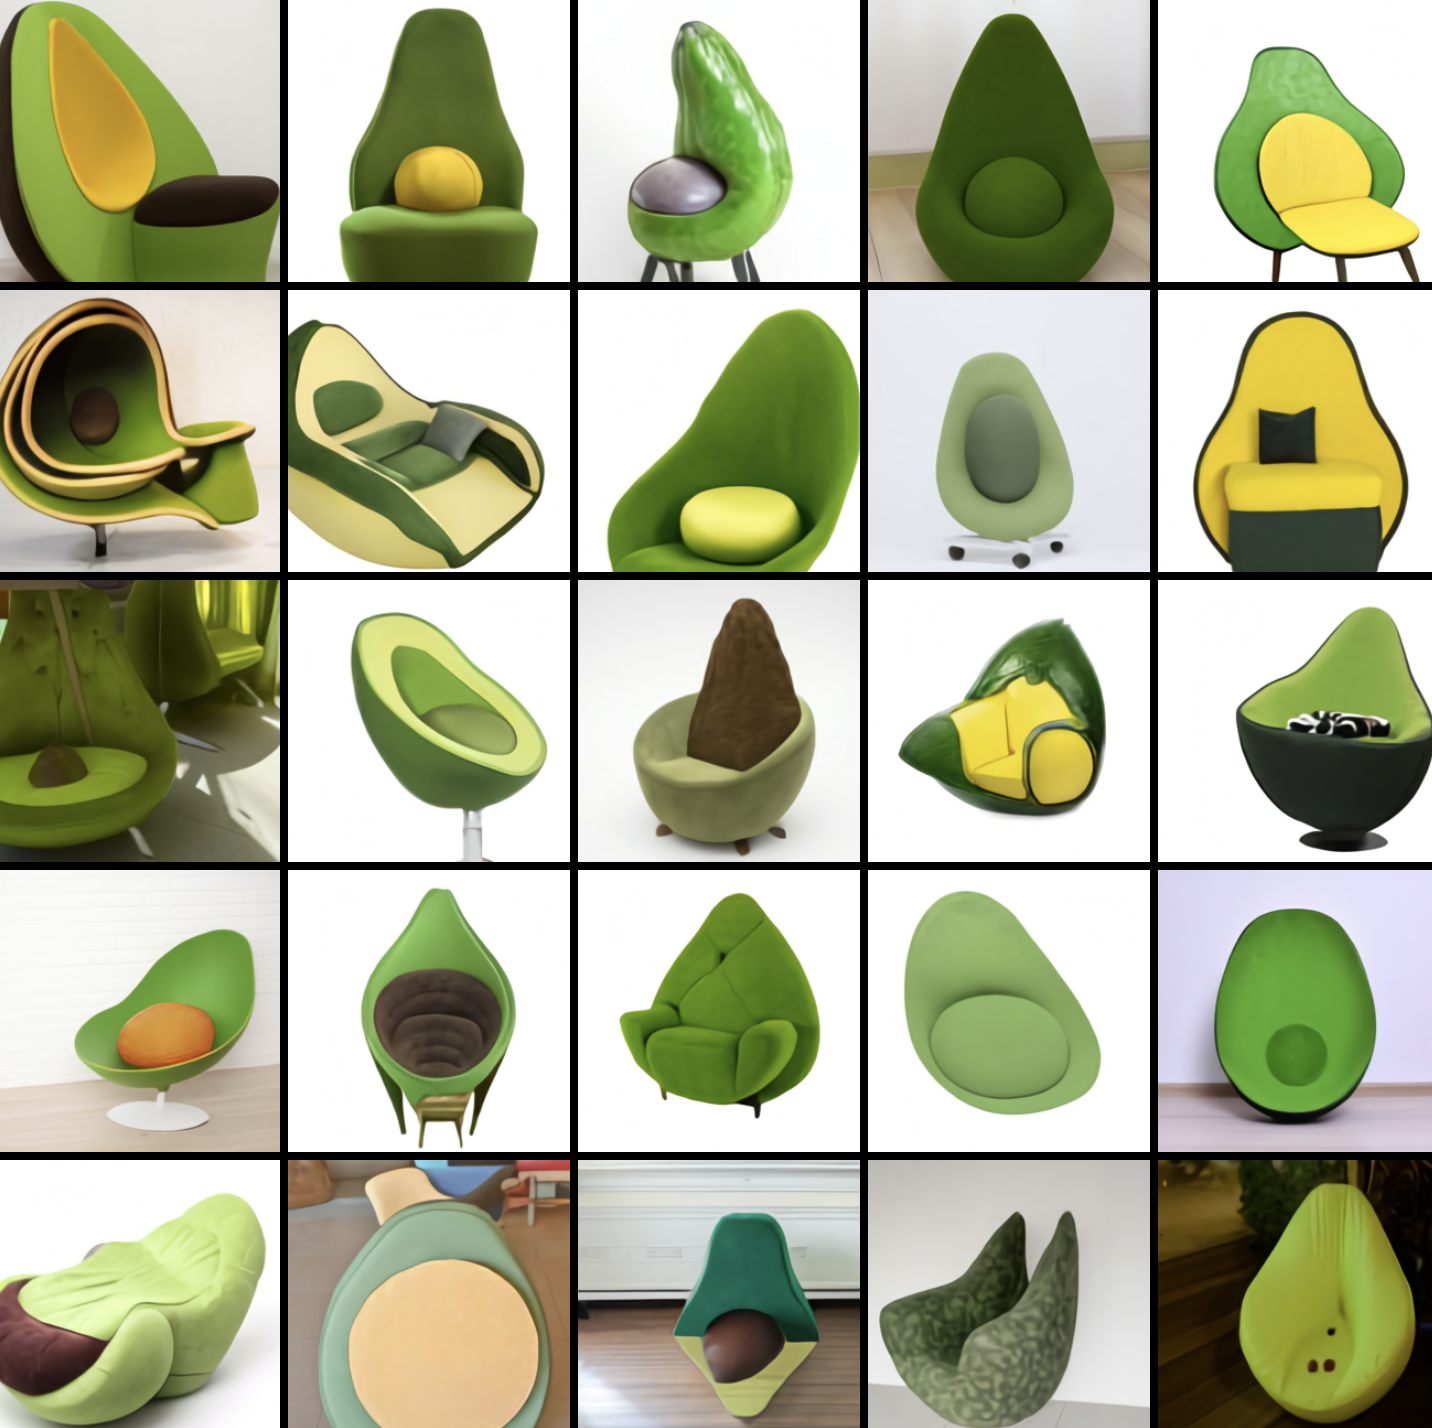
\includegraphics[scale=0.2]{dalle_avocado.png}
\end{figure} 
\end{frame}

\section{Theory}

\begin{frame}[c]{GANs - Generic Adversarial Networks}
\begin{columns}[t]
  \begin{column}{0.5\linewidth}
  \begin{block}{BigGAN}
   
   \end{block}
  \end{column}
   \begin{column}{0.5\linewidth}
  \begin{block}{StyleGAN}
\begin{figure}[ht!]
    \centering
    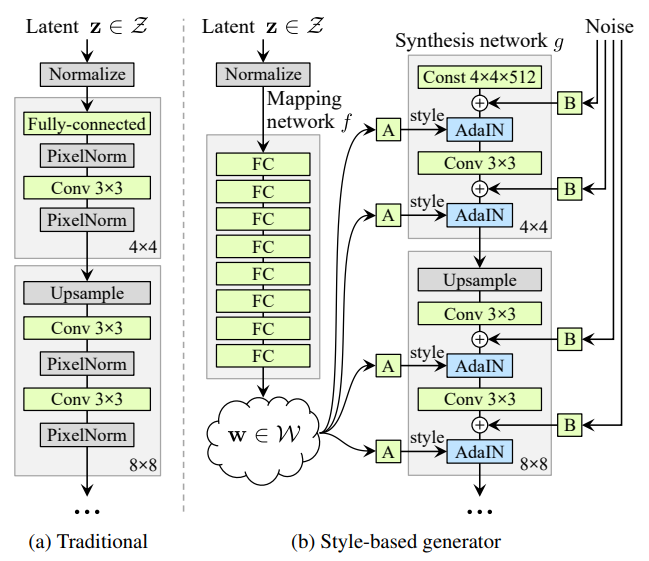
\includegraphics[scale=0.2]{stylegan-scheme.PNG}
\end{figure} 
   \end{block}
  \end{column}
 \end{columns}
\end{frame}

\begin{frame}{CLIP}
\textbf{CLIP} - Contrastive Language-Image Pre-Training new multi-modal model released by OpenAI in January 2021.  \\
Key features:
\begin{itemize}
\item it is a neural network trained on over $400 \; 000 ; 000$ (image, caption) pairs
\item main usage is to obtain the most relevant text snipper for given image
\end{itemize}
\begin{figure}[ht!]
    \centering
    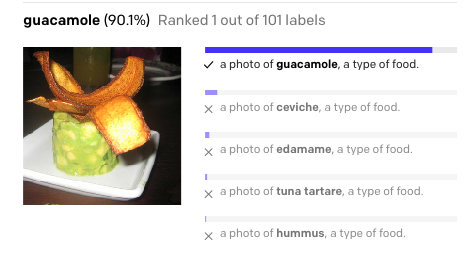
\includegraphics[scale=0.5]{clip_example.png}
\end{figure} 
\end{frame}
\begin{frame}{Evolutionary Algorithms}

\begin{block}{Genetic Algorithm}
\begin{figure}[ht!]
    \centering
    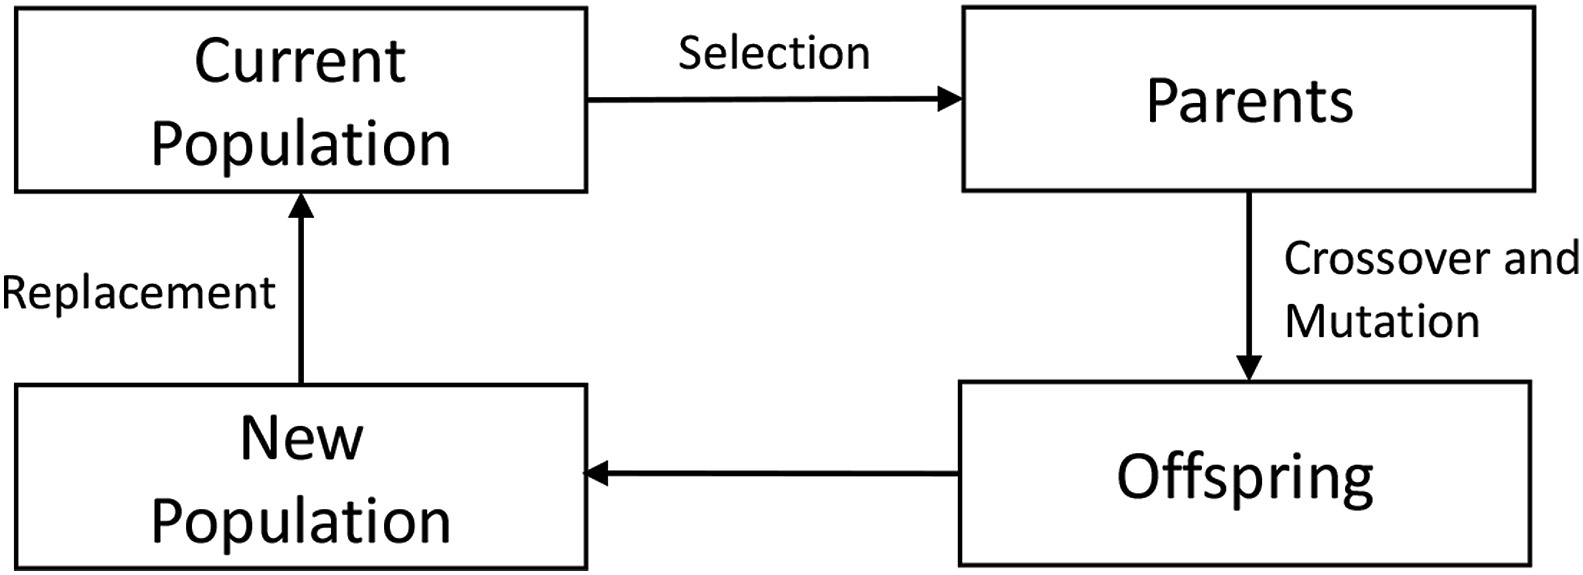
\includegraphics[scale=0.5]{gen-algo.jpg}
\end{figure} 
\end{block}

\begin{block}{Differential Evolution}
\end{block}

\end{frame}

\section{Framework}

\begin{frame}{Framework}
\begin{figure}[ht!]
    \centering
    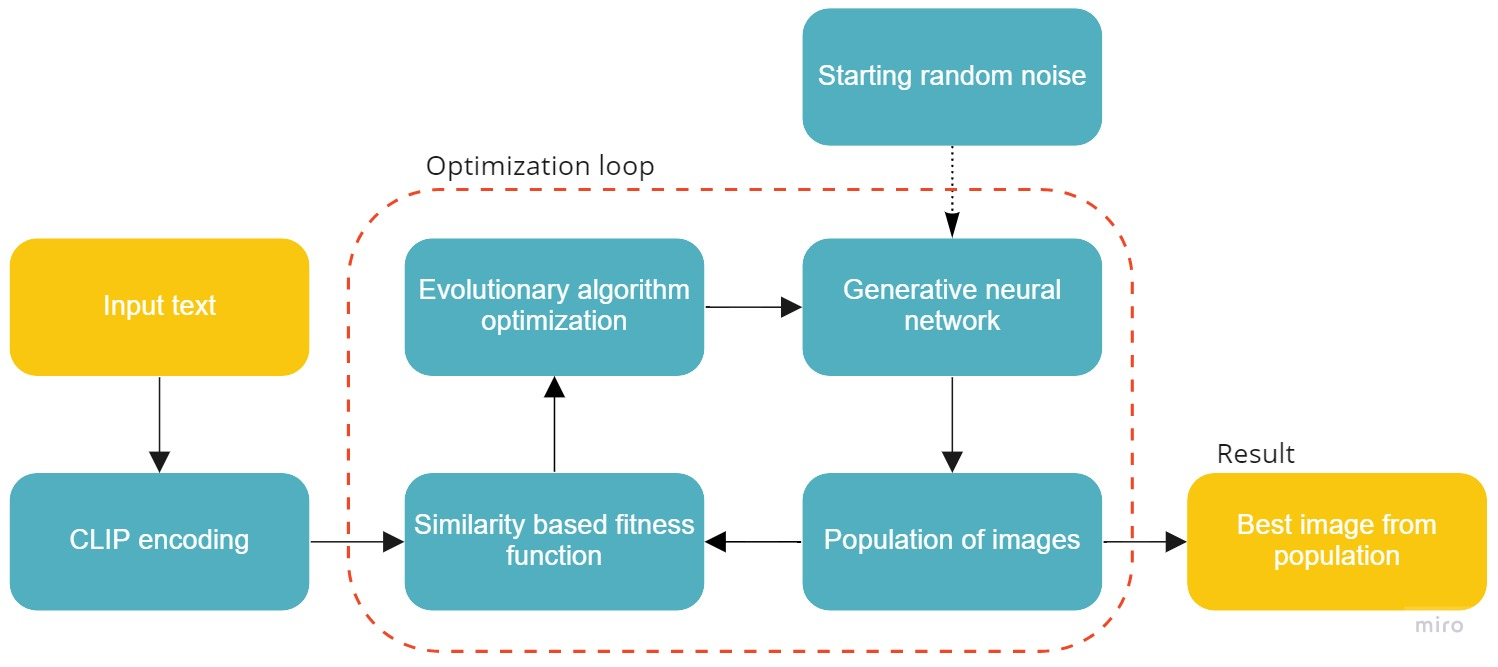
\includegraphics[scale=0.2]{framework.jpg}
\end{figure} 
\end{frame}

\section{Best Results}

\begin{frame}[c]{Best Results}
\begin{figure}[ht!]
    \centering
    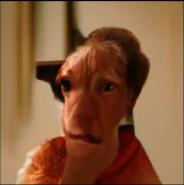
\includegraphics[scale=0.8]{best.png}
\end{figure} 
\end{frame}

\section{Experiments}

\begin{frame}{Evaluation - CIFAR10}
\begin{table}[h!]
\centering
\begin{tabular}{|l|c|c|c|}
\hline
\multicolumn{1}{|c|}{\textbf{Class}} & \textbf{Positive} & \textbf{Negative} & \textbf{Accuracy (\%)}       \\ \hline
AIRPLANE                             & 476               & 36                & {\color[HTML]{32CB00} 92.97} \\ \hline
AUTOMOBILE                           & 88                & 424               & 17.19                        \\ \hline
BIRD                                 & 12                & 500               & 2.34                         \\ \hline
CAT                                  & 177               & 335               & 34.57                        \\ \hline
DEER                                 & 0                 & 512               & {\color[HTML]{FE0000} 0.0}   \\ \hline
DOG                                  & 255               & 257               & 49.8                         \\ \hline
FROG                                 & 39                & 473               & 7.62                         \\ \hline
HORSE                                & 64                & 448               & 12.5                         \\ \hline
SHIP                                 & 60                & 452               & 11.72                        \\ \hline
TRUCK                                & 97                & 415               & 18.95                        \\ \hline
\textbf{TOTAL}                       & \textbf{1268}     & \textbf{3852}     & \textbf{24.77}               \\ \hline
\end{tabular}
\end{table}
\end{frame}

\begin{frame}[c]{Evaluation - CIFAR10}
\begin{figure}
    \centering
    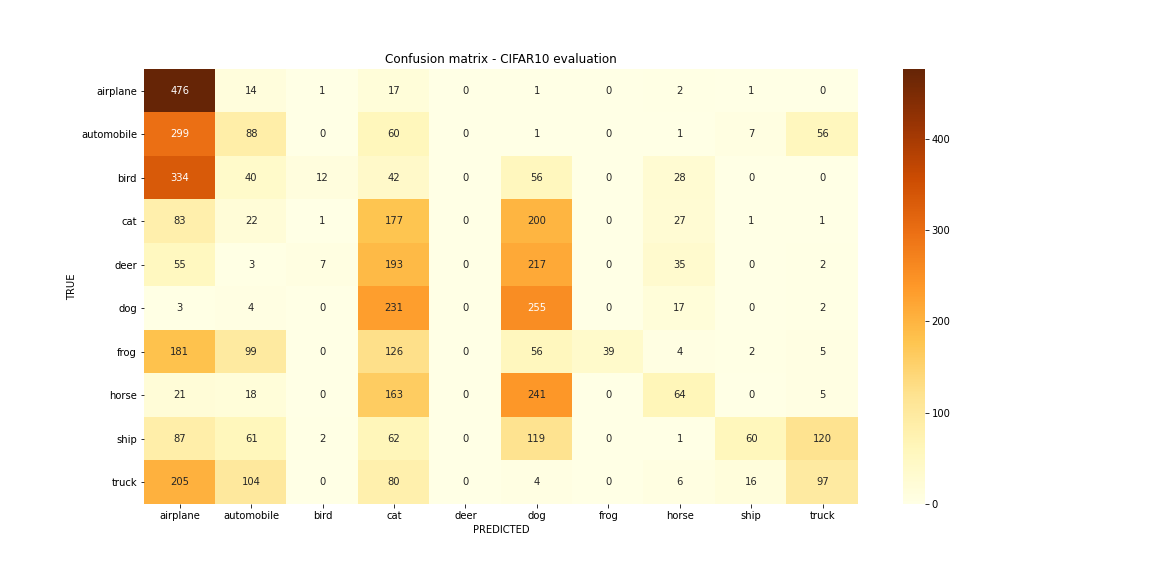
\includegraphics[scale=0.3]{confusion_matrix.png}
\end{figure} 
\end{frame}

\begin{frame}[c]{Evaluation - CIFAR10 - Example}
\textbf{Airplane}
\begin{figure}
    \centering
    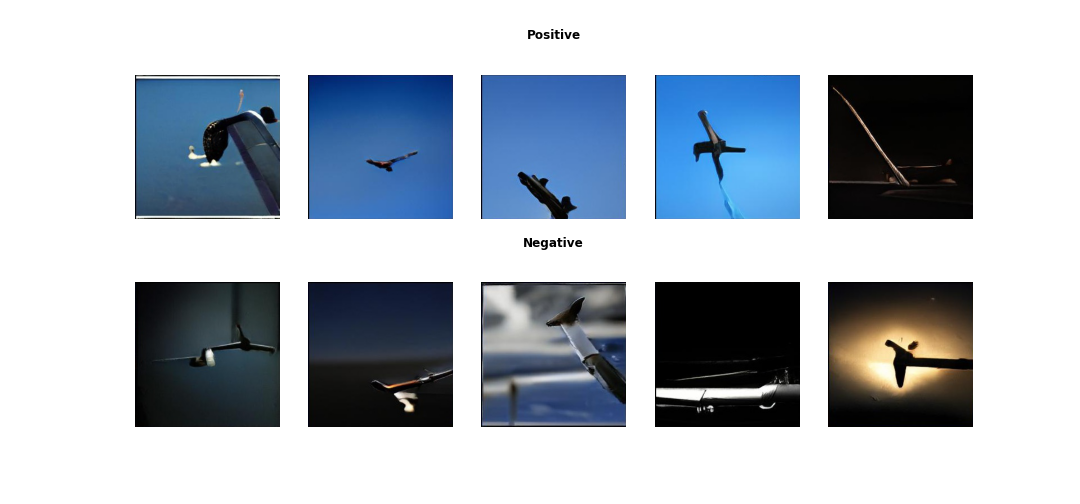
\includegraphics[scale=0.25]{airplane.png}
\end{figure} 
\end{frame}

\begin{frame}[c]{Evaluation - ImageNet}
\fontsize{10}{7.2}\selectfont
\begin{table}[h!]
\begin{tabular}{|l|c|c|c|}
\hline
\multicolumn{1}{|c|}{\textbf{Class}} & \textbf{Positive} & \textbf{Negative} & \textbf{Accuracy (\%)}       \\ \hline
BANANA                               & 111               & 401               & {\color[HTML]{000000} 21.68} \\ \hline
CASH MACHINE                         & 124               & 388               & 24.22                        \\ \hline
HAMMER                               & 141               & 371               & 27.54                        \\ \hline
ICE CREAM                            & 3                 & 509               & {\color[HTML]{FE0000} 0.59}  \\ \hline
LLAMA                                & 36                & 476               & {\color[HTML]{333333} 7.03}  \\ \hline
MINISKIRT                            & 220               & 292               & 42.97                        \\ \hline
PIRATE                               & 5                 & 507               & 0.98                         \\ \hline
SHOPPING CART                        & 125               & 387               & 24.41                        \\ \hline
WALL CLOCK                           & 146               & 366               & 28.52                        \\ \hline
KERRY BLUE TERRIER                   & 253               & 259               & {\color[HTML]{32CB00} 49.41} \\ \hline
\textbf{TOTAL}                       & \textbf{1164}     & \textbf{3956}     & \textbf{22.73}               \\ \hline
\end{tabular}
\end{table}
\end{frame}

\begin{frame}[c]{Evaluation - ImageNet - Example}
\textbf{Llama}
\begin{figure}
    \centering
    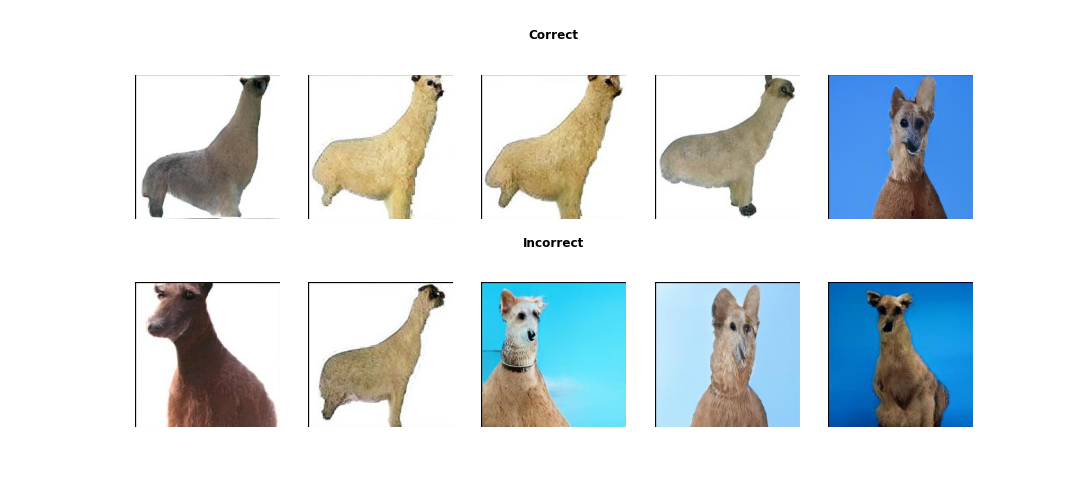
\includegraphics[scale=0.25]{llama.png}
\end{figure} 
\end{frame}

\begin{frame}{GA vs DE}
\begin{figure}[h]
    \centering
    \subfloat[\centering genetic algorithm]{{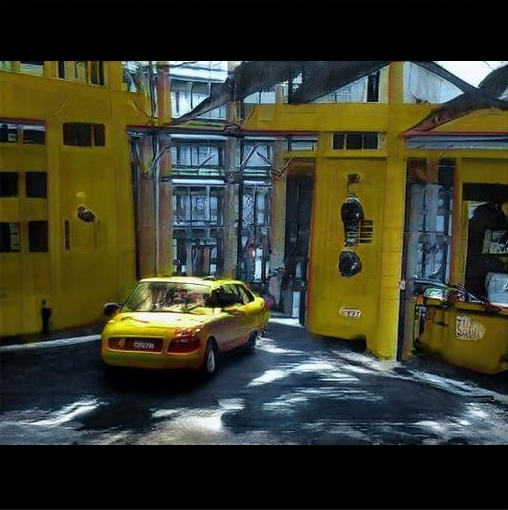
\includegraphics[width=3cm]{GA_yellowcar_final.PNG} }}
    \qquad
    \subfloat[\centering differential evolution]{{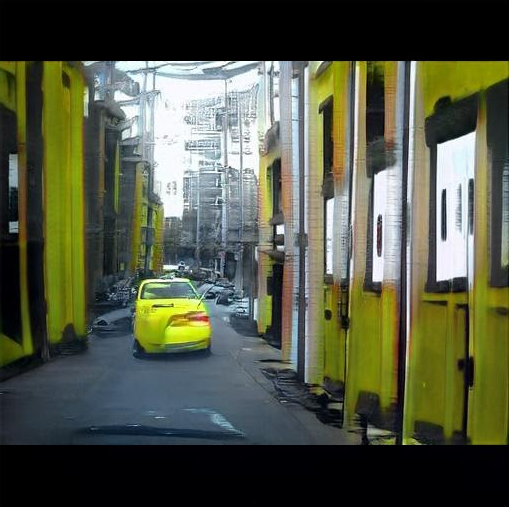
\includegraphics[width=3cm]{DE_yellowcar_final.PNG} }}
    \caption{Final images (with best score) produced by algorithms.}
\end{figure}
\end{frame}

\begin{frame}[c]{BigGAN vs StyleGAN}
...
\end{frame}

\begin{frame}{Cosine-Similarity}
Observations:
\begin{itemize}
\item \textit{cos-sim} in our solution takes values only in the range $\sim [0.2, 0.4]$
\end{itemize}
\begin{figure}
    \centering
    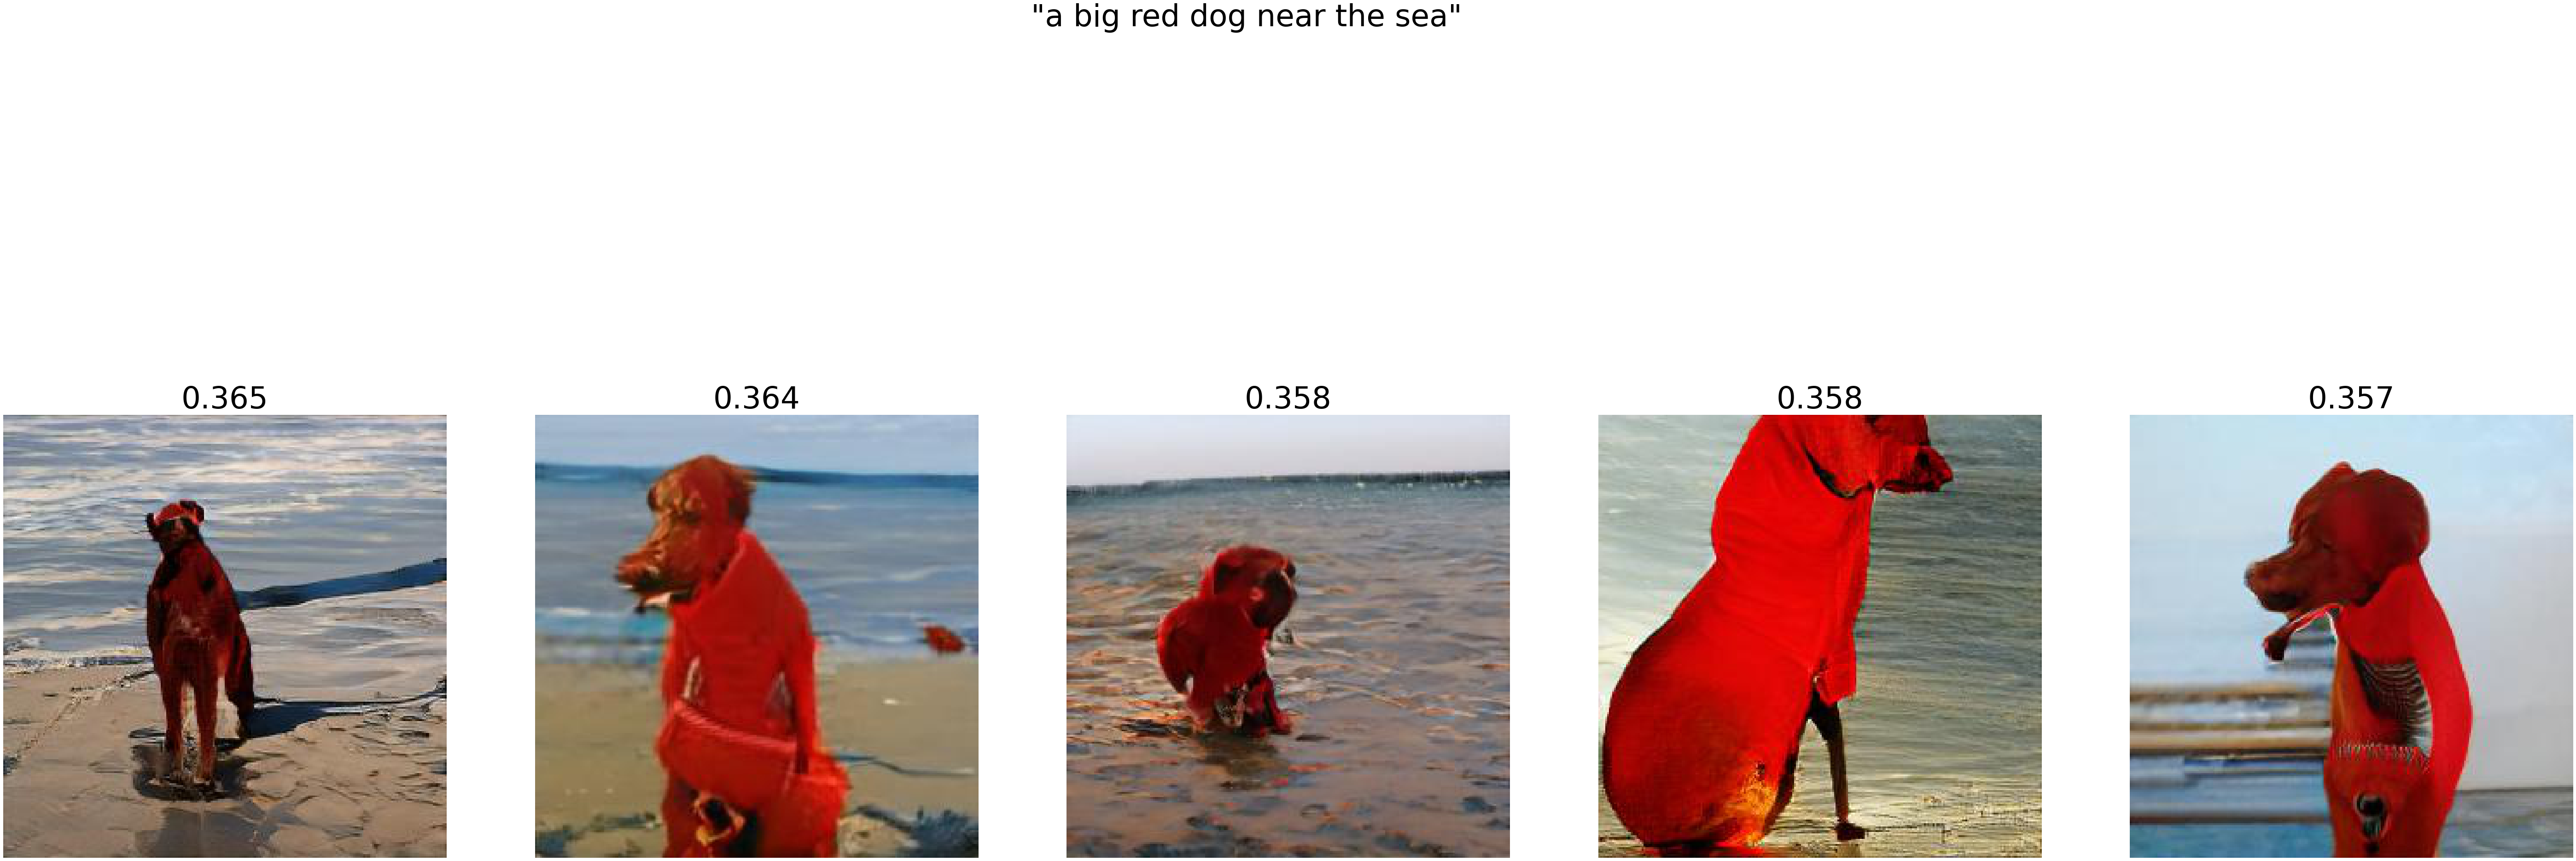
\includegraphics[scale=0.05]{bigreddog.png}
\end{figure} 
\end{frame}

\section{Conclusions}

\begin{frame}[c]{Conclusions}
\begin{itemize}
\item A
\item B
\item C
\end{itemize}
\end{frame}

\section{Bibliography}

\begin{frame}{Bibliography}
\fontsize{2}{7.2}\selectfont
\begin{thebibliography}{a,b,c}
\addcontentsline{toc}{chapter}{Citation}
\bibitem[1]{improvedgans} T. Salimans, I. Goodfellow, W. Zaremba, V. Cheung, A. Radford, and X. Chen. {\it Improved techniques for training gans.} In NIPS, 2016.

\bibitem[2]{inception} C. Szegedy, V. Vanhoucke, S. Ioffe, J. Shlens, Z. Wojna. {\it Rethinking the inception architecture for computer vision.} arXiv preprint arXiv: 1512.00567, 2015.

\bibitem[3]{noteonis} S. Barratt, R. Sharma. {\it A note on the Inception Score.} arXiv preprint arXiv: 1801.01973, 2018.

\bibitem[4]{fid} M. Heusel, H. Ramsauer, T. Unterthiner, B. Nessler, S. Hochreiter. {\it GANs trained by a two time-scale update rule converge to a local Nash equilibrium.} In NIPS, 2017.

\bibitem[5]{de} R. Storn, K. Price. {\it Differential Evolution – A Simple and Efficient Heuristic for global Optimization over Continuous Spaces.} Springer, 1997.

\bibitem[6]{stylegan} T. Karras, S. Laine, T. Aila. {\it A style-based generator architecture for generative adversarial networks.} In CVPR, 2019.

\bibitem[7]{gan} I. Goodfellow et al.  {\it Generative Adversarial Nets} 2014.  \url{https://arxiv.org/pdf/1406.2661.pdf}

\bibitem[8]{ganprogress} M. Brundage, S. Avin, J. Clark et al. {\it The Malicious Use of Artificial Intelligence: Forecasting, Prevention, and Mitigation.} arXiv preprint arXiv: 1802.07228, 2018.

\bibitem[9]{clip} OpenAI CLIP https://arxiv.org/pdf/2103.00020.pdf

\bibitem[10]{cifar10_data} https://www.cs.toronto.edu/~kriz/cifar.html

\bibitem[11]{imagenet_data} https://www.image-net.org/

\bibitem[12]{clip} A. Radford, J. W. Kim, C. Hallacy, A. Ramesh, G. Goh, S. Agarwal, G. Sastry, A. Askell, P. Mishkin, J. Clark et al. {\it Learning transferable visual models
from natural language supervision.} In CVPR, 2019.

\bibitem[13]{clip_blog} https://openai.com/blog/clip/

\bibitem[14]{clip_source} https://habr.com/en/post/537334/

\bibitem[15]{cifar10_classifier} \url{https://github.com/vrakesh/CIFAR-10-Classifier}

\bibitem[16]{resnet} \url{https://pytorch.org/hub/pytorch_vision_resnet}

\bibitem[17]{imagenet_example} \url{https://devopedia.org/imagenet}

\bibitem[18]{gan_arch} \url{https://machinelearningmastery.com/what-are-generative-adversarial-networks-gans/}

\end{thebibliography}
\end{frame}
\end{document}
